\documentclass{beamer}

\usecolortheme[light]{solarized}

\beamertemplatenavigationsymbolsempty

\usepackage{hyperref}
\usepackage{minted}

\usepackage{graphicx}
\usepackage{tikz}

\usetikzlibrary{calc, patterns}

\begin{document}

    \begin{frame}
        \begin{center}
            \Huge

            Waiting lines, queues and ciw.

            \Large

            \href{https://twitter.com/drvinceknight}
            {@drvinceknight}


            \href{https://github.com/CiwPython/Ciw}
            {github.com/CiwPython/Ciw}

            \vfill

            
\includegraphics[width=.3\textwidth]{./assets/ciw-logo.png}

        \end{center}
    \end{frame}

    \begin{frame}
        \begin{center}
            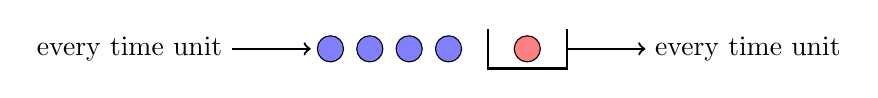
\begin{tikzpicture}

                \node (I1) at (0, 0) [draw, circle, fill=blue!50] {};
                \node (I2) at ($(I1) + (0.5, 0)$) [draw, circle, fill=blue!50] {};
                \node (I3) at ($(I2) + (0.5, 0)$) [draw, circle, fill=blue!50] {};
                \node (I4) at ($(I3) + (0.5, 0)$) [draw, circle, fill=blue!50] {};

                \draw ($(I1) + (-1.25, 0)$) -- ($(I1) + (-.25, 0)$) [->, thick] ;
                \node at ($(I1) + (-1.25, 0)$) [left] {every time unit};

                \draw [thick] ($(I4) + (0.5, 0.25)$) --
                              ($(I4) + (0.5, -0.25)$) --
                              ($(I4) + (1.5, -0.25)$) --
                              ($(I4) + (1.5, 0.25)$);

                \node (I5) at ($(I4) + (1, 0)$) [draw, circle, fill=red!50] {};

                \draw ($(I5) + (.5, 0)$) -- ($(I5) + (1.5, 0)$) [->, thick];
                \node at ($(I5) + (1.5, 0)$) [right] {every time unit};


            \end{tikzpicture}
        \end{center}
    \end{frame}

    \begin{frame}[fragile]{}
        \begin{minted}{python}
>>> import ciw
>>> dist = ['Deterministic', 1]
>>> N = ciw.create_network(Arrival_distributions=[dist],
...                        Service_distributions=[dist],
...                        Number_of_servers=[1])
>>> seed = 0
>>> max_customers = 5000
>>> ciw.seed(seed)
>>> Q = ciw.Simulation(N)
>>> Q.simulate_until_max_customers(max_customers)

        \end{minted}
\end{frame}

    \begin{frame}[fragile]{}
        \begin{minted}{python}
>>> Q.nodes
[Arrival Node, Node 1, Exit Node]
>>> Q.nodes[-1].all_individuals[6].data_records
[Record(...arrival_date=7, ...service_start_date=7...)]

        \end{minted}
\end{frame}

    \begin{frame}[fragile]{}
        \begin{minted}[fontsize=\footnotesize]{python}
>>> def get_times(Q):
...     """
...     Obtain total time and service time of every individual
...     """
...
...     total_times = [ind.data_records[0].exit_date -
...                    ind.data_records[0].arrival_date
...                    for ind in Q.nodes[-1].all_individuals[:-1]]
...     service_times = [ind.data_records[0].service_time
...                      for ind in Q.nodes[-1].all_individuals[:-1]]
...     return total_times, service_times

>>> total_times, service_times = get_times(Q)

        \end{minted}
\end{frame}

\begin{frame}
    \begin{center}
        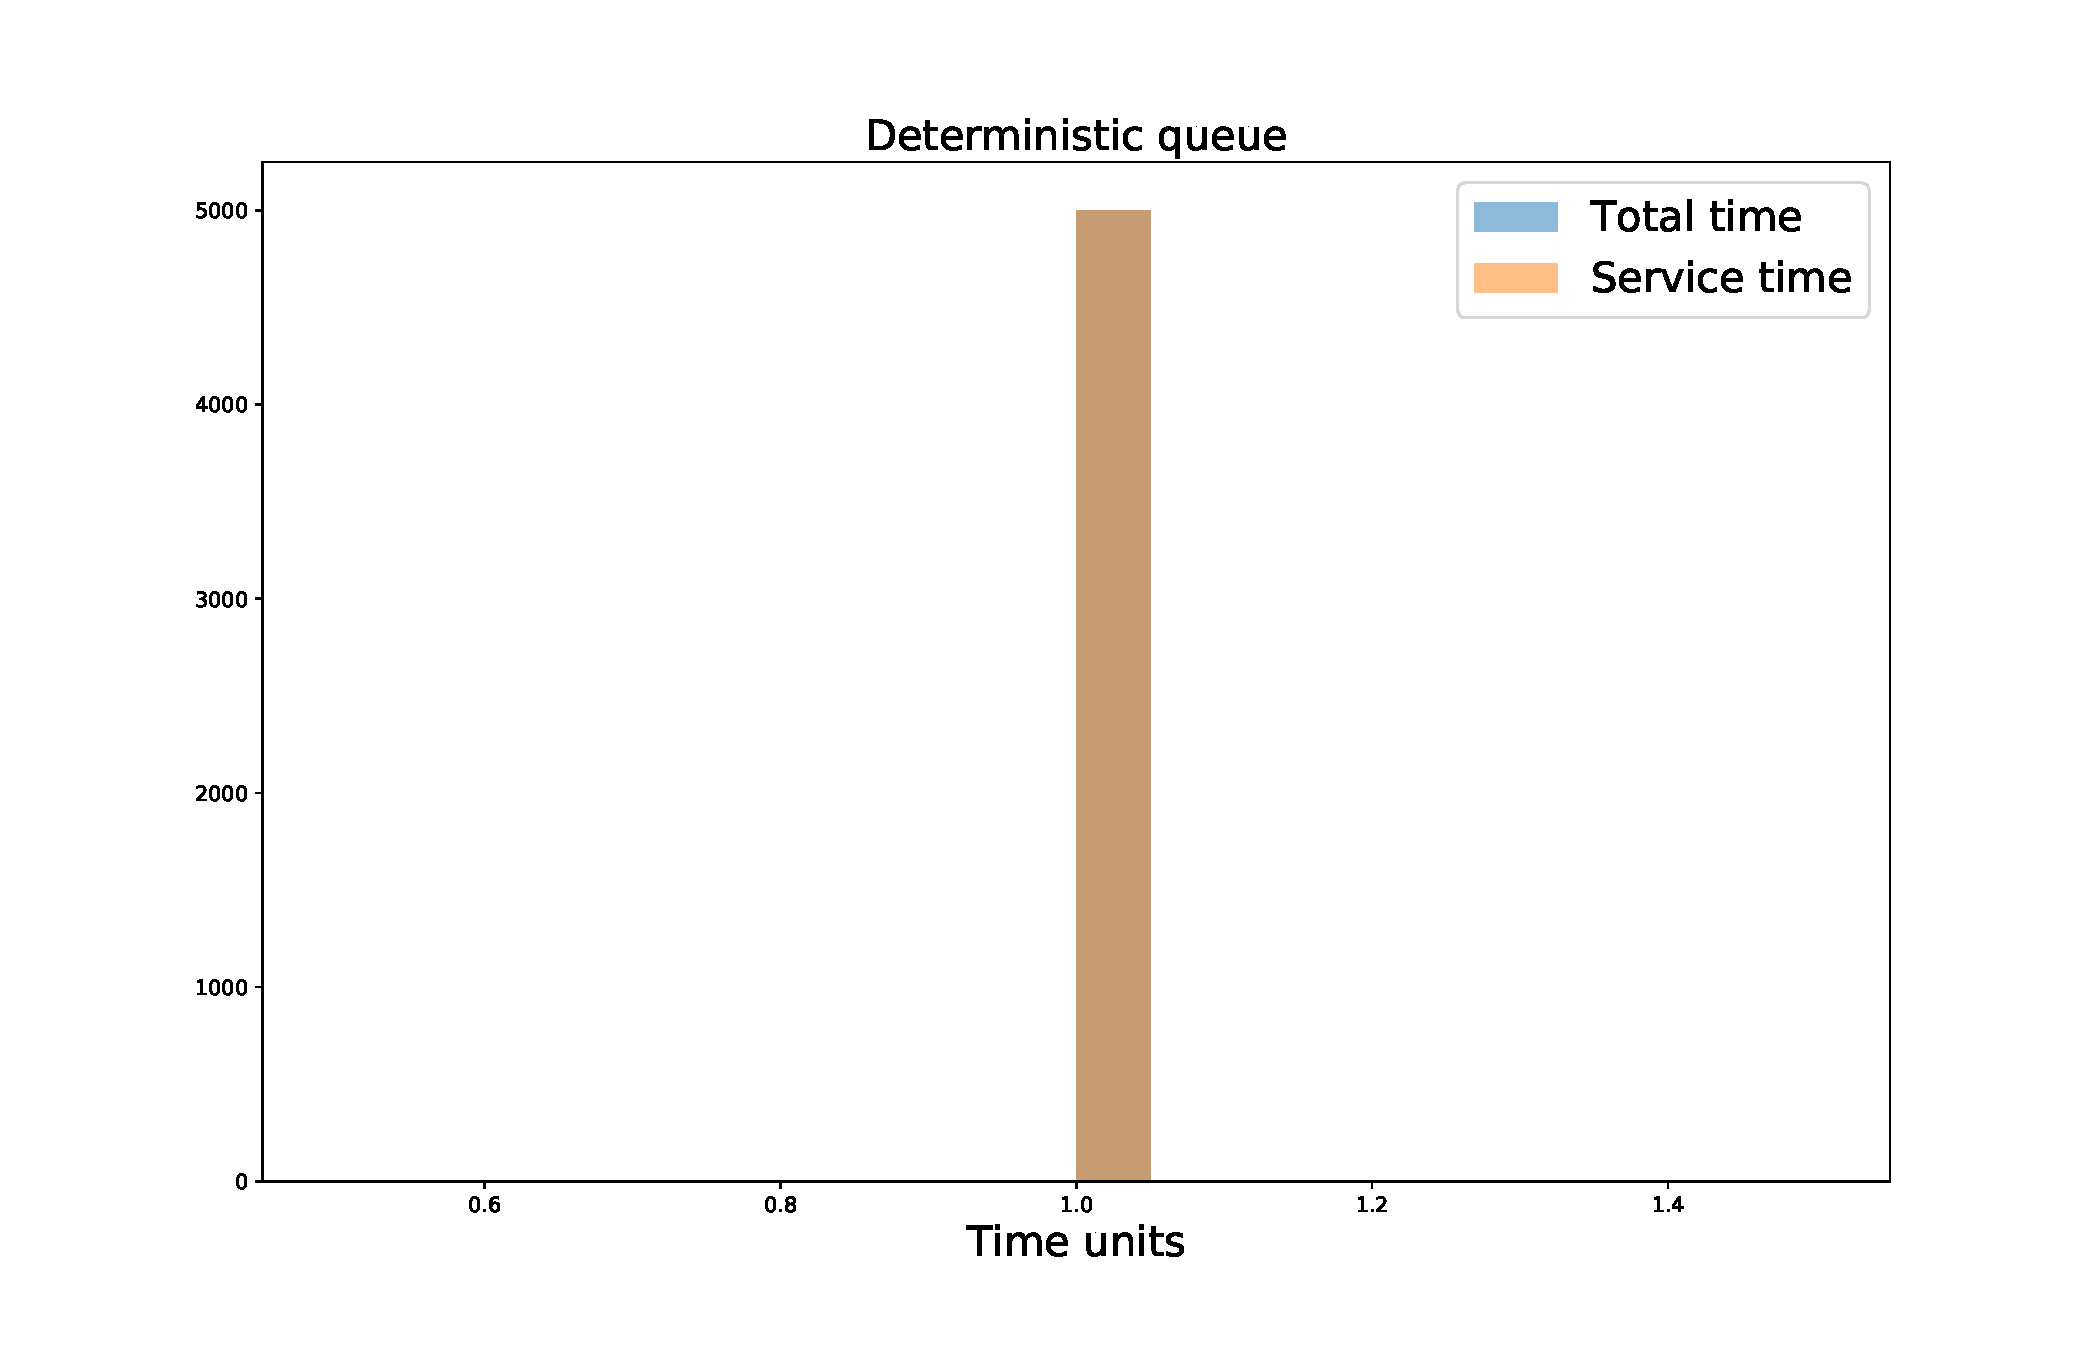
\includegraphics[width=\textwidth]{assets/deterministic_queue.pdf}
    \end{center}
\end{frame}

    \begin{frame}[fragile]{}
        \begin{minted}{python}
>>> dist = ['Exponential', 1]
>>> N = ciw.create_network(Arrival_distributions=[dist],
...                        Service_distributions=[dist],
...                        Number_of_servers=[1])
>>> seed = 0
>>> max_customers = 5000
>>> ciw.seed(seed)
>>> Q = ciw.Simulation(N)
>>> Q.simulate_until_max_customers(max_customers)
>>> total_times, service_times = get_times(Q)

        \end{minted}
\end{frame}

\begin{frame}
    \begin{center}
        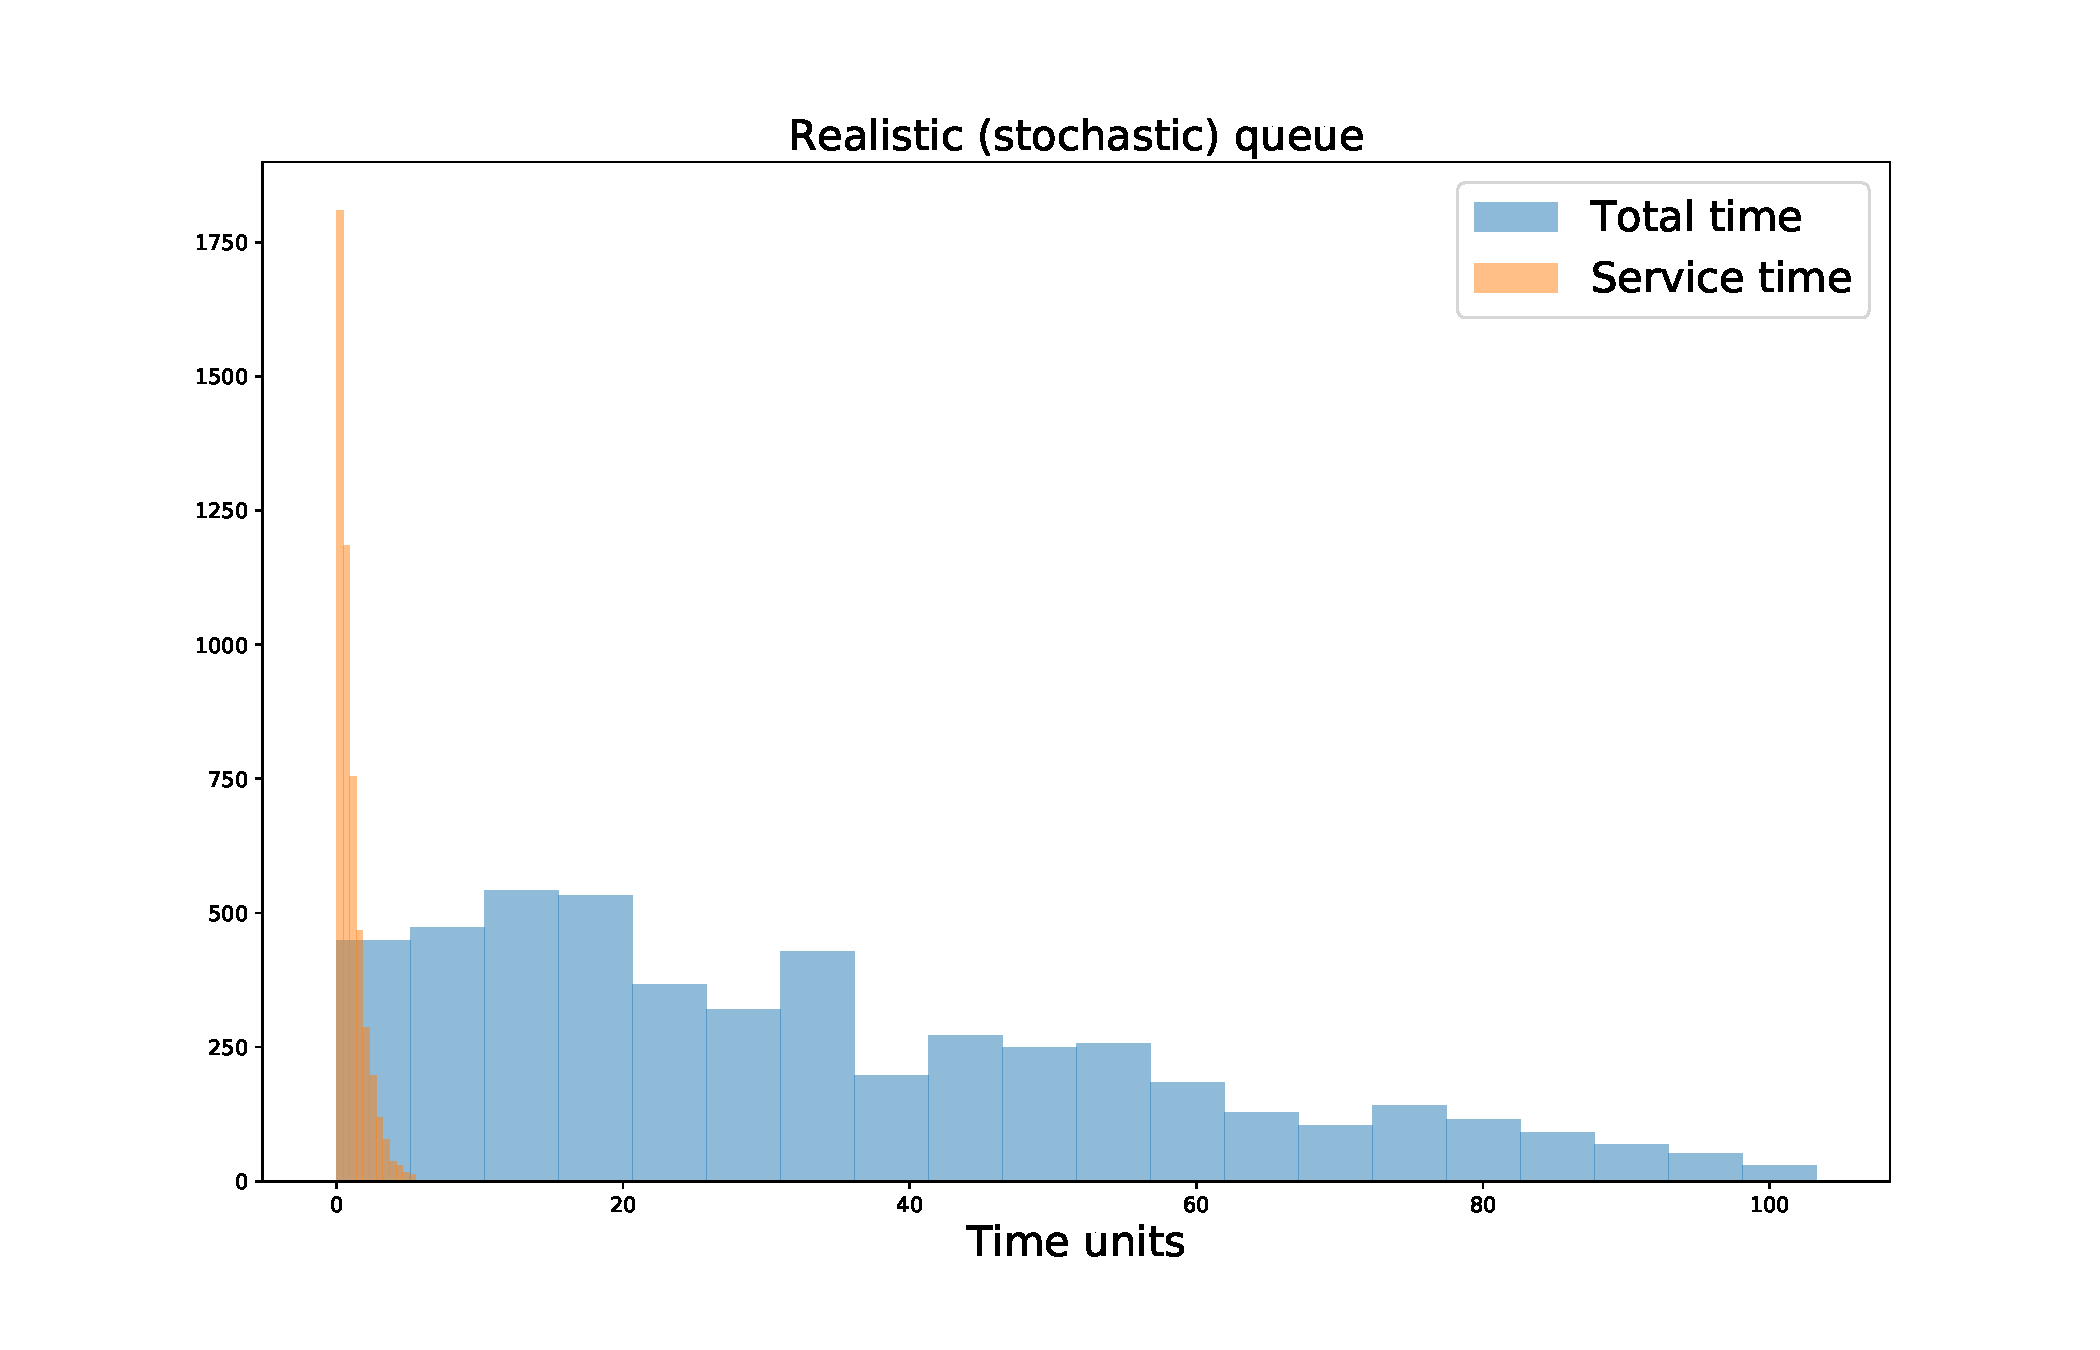
\includegraphics[width=\textwidth]{assets/stochastic_queue.pdf}

        \pause
        \Large
            \href{https://github.com/CiwPython/Ciw}
            {github.com/CiwPython/Ciw}
    \end{center}
\end{frame}

\end{document}
